\documentclass[11pt]{article} 

%\usepackage{float}
%\usepackage{algorithm2e}
%\usepackage{algorithmic}
\usepackage{amsmath}
\usepackage{amsthm}
\usepackage{booktabs}
\usepackage{caption}
\usepackage{dcolumn}
\usepackage{epstopdf}
\usepackage{fourier}
\usepackage{fullpage}
\usepackage{graphicx}
\usepackage{hyperref}
\usepackage{longtable}
\usepackage{multirow}
\usepackage{nag}
\usepackage{natbib}
\usepackage{pdflscape}
\usepackage{rotating}
\usepackage{setspace}
\usepackage{subfig}
\usepackage{tabularx} 
\usepackage{tikz} 
\usepackage{url}

\hypersetup{
  colorlinks, 
  citecolor=blue, 
  filecolor=blue, 
  linkcolor=red, 
  urlcolor=blue, 
pdftex}

\DeclareMathOperator*{\argmax}{arg\,max}
%\newcommand{\starlanguage}{Significance indicators: $p \le 0.05:*$, .$p \le 0.01:**$ and $p \le .001:***$.}  
\newcommand{\starlanguage}{Significance indicators: $p \le 0.10:*$,
  .$p \le 0.05:**$ and $p \le .01:***$.}  
\newtheorem{proposition}{Proposition}
\newtheorem{assumption}{Assumption}
\newtheorem{lemma}{Lemma}

\begin{document}

\title{Are Online Labor Markets Spot Markets for Tasks?:\\ A Field
  Experiment on the Behavioral Response to Wage Cuts\footnote{
The authors thank Kelsey Jack, Nolan Miller, Jeffrey Liebman and Richard Zeckhauser for helpful discussions.
Work on this project was conducted while Daniel Chen received financal support from the Institute for Humane Studies, the John M. Olin Foundation, and the Petrie-Flom Center.
John Horton received financial support from the Harvard Multidisciplinary Program in Inequality \& Social Policy.
Both authors gratefully acknowledge funding from the Berkman Center for Internet and Society at Harvard Law School. A draft of this paper previously circulated under the title ``The Wages of Paycuts.''
}} 

\author{Daniel L. Chen\\Toulouse Institute for Advanced Study \and John J. Horton\\NYU Stern}

\date{}
\maketitle{}

\begin{abstract} 
  \noindent
  In some online labor markets, workers are paid by the task, choose what tasks to work on, and have little or no interaction with their (usually anonymous) buyer/employer.  
  These markets look like true spot markets for tasks rather than markets for employment. 
  Despite appearances, we find via a field experiment that workers act more like parties to an employment contract:
  workers quickly form wage reference points and react negatively to proposed wage cuts by quitting.
  However, they can be mollified with ``reasonable'' justifications for why wages are being cut, highlighting the importance of fairness considerations in their decision making. 
  We find some evidence that ``unreasonable'' justifications for wage
  cuts reduce subsequent work quality. 
  We also find that not explicitly presenting the worker with a decision about continuing to work eliminates ``quits,'' with no apparent reduction in work quality.
  One interpretation for this finding is that workers have a strong expectation that they are party to a quasi-employment relationship where terms are not changed, and the default behavior is to continue working. 
  \newline \newline 
Keywords: Economics of IS; Electronic Commerce; Field Experiments; IT and new organizational forms
% JEL Codes: J30, D03, D63 \newline \newline 
\end{abstract} 

\doublespacing

\section{Introduction}
According to \cite{coase1937nature}, the boundary of the firm is determined by the relative costs and benefits of organizing production through markets or through authority. 
For the labor input to production, this markets-versus-authority choice was conceptualized by \cite{simon1951formal} as the choice between what Simon called a ``sales contract'' and the conventional employment contract.
In Simon's model, the employee accepts a wage in exchange for giving the employer control over what precise \emph{task}, from some set of tasks, is done in the future.
While employment is at will, the expectation is that the relationship will be ongoing and persist until explicitly dissolved. 
In contrast, a sales contract is narrower in scope, with the worker agreeing to complete a specific task for a specific price.
When the task is completed and payment made, the contract is dissolved. 
Simon's labels are not always easy to apply (e.g., consider the salesperson who works on commission), but the number of edge cases seems to have grown dramatically in recent years with the emergence of new labor-intermediating platforms. 
Platforms differ, but a number seem to create quasi-employment or quasi-sales contracts that share features of both types of relationships.\footnote{
An example of a technology-driven platform creating this kind of confusion is Uber.  
Uber sets ride prices and determines who is eligible to drive, but does not tell drivers which precise customer to pick up or when to work---but it does impose standards of performance.
Perhaps unsurprisingly, a number of worker classification lawsuits have sprung up around this industry.
}

One kind of new labor-intermediating platform of particular interest is the online labor market \citep{horton2010online}. 
In the case of online labor markets, some create relationships that at least have some of the properties of traditional employment relationships:
workers are paid by the hour, and projects can be substantial and may require a number of different tasks, with the work being closely monitored by the hiring firm.
Examples from this mold include oDesk/Elance (now Upwork), Freelancer.com, Guru, and several other more specialized sites. 
However, other online labor markets are far more task focused and seemn to create sales contract relationships.

The most extreme version of a task-focused market is Amazon Mechanical Turk (MTurk), where tasks often take seconds and pay pennies.
``Employers'' in this market cannot exercise Simon-style authority, because they do not communicate with workers (except initially, through the job description)---workers simply and immediately complete the task at the terms proposed by the buyer.
Workers are free to take any task they want at the offered price. 
This market, at least based on its main characteristics, seems like a true spot market for tasks.
If this is the case, MTurk and markets like it would offer firms a profoundly different way of obtaining labor inputs. 
With a spot market, firms could buy discrete chunks of labor from a global pool of workers at a market price, similar to how they obtain any other factor of production.   

Even if MTurk is conceptualized by employers and Amazon itself as a spot market in tasks, this does not imply that workers share this view or behave accordingly. 
In this paper, we test whether workers on MTurk react as parties to a sales contract or an employment contract when presented with a wage cut. 
We conducted an experiment in which we contracted with workers for a data-entry task, paid them a high piece rate and then offered some treated workers the opportunity to keep working, albeit for a lower rate. 
While in both the sales contract and employment characterizations fewer workers should be willing to accept the lower offer, the two views differ in how ``justifications'' for the new offer should affect worker uptake.

For a party to a sales contract in a spot market, how price changes are justified is materially irrelevant and should not differentially affect uptake of the follow-on task.
However, for a party to an employment contract, a lower offer would be perceived as a wage cut, which in turn could provoke retaliation from the worker, depending on the perceived justice of that offer. 
We designed the different framings and justifications so that they would provoke workers to view the cuts as either reasonable and fair or capricious and unjust.\footnote{ 
  While we technically were offering a lower piece rate rather than a chance in time-based compensation, we refer throughout to the text as a ``wage cut.''
  }
 
Consistent with the employment view, but not the spot market view, we find that workers were more likely to reject low offers, but justifications we deemed ``reasonable'' largely nullified this effect. 
Not all justifications were effective---justifying the cut in terms of our profits actually increased quits (i.e., individuals unwilling to perform a follow-on task at the new offer). 

A worker's quality might suffer following a wage cut. 
We can only measure work quality for people who actually accepted the wage cut and performed an additional task. 
As such, it is possible that different kinds of workers quit in different treatments, so differences in quality across treatments could simply reflect selection effects as well as treatment effects.
However, when we control for work quality from the first stage, we do find evidence of lower quality in the ``profits'' treatments, suggesting the possibility of retaliation. 

In each of the different testing justifications for the new offer, we still explicitly framed the decision about whether to continue working as a choice, with the new per-task payment made salient.
However, in one cell, we simply presented another data entry task with the new wage cut price clearly labeled, but without an explicit framing of a new offer and the need for a worker decision.
In this cell, 100\% of workers simply completed the next paragraph---a higher percentage than when they were offered their previous wage.  
Worker mistake is a possibility---perhaps they believed that not completing our extra paragraph would jeopardize payment---but we find no evidence of follow-on retaliation in this group.
A parsimonious explanation could be that workers regard themselves as being in quasi-employment relationships and so the ``default'' is to simply keep working without the expectation of---or the need for---renegotiation.   

The evidence from the experiment suggests that even in the most ``spot'' of the online labor markets, workers still bring an employee-like behavior to their interactions.
MTurk is, of course, only one market and the results of the experiment come from a self-selected sample of workers on that market.
It is necessarily unclear whether these results would extend to other markets and other kinds of workers.
However, given that MTurk is the most spot-market like in its observable characteristics, it seems probable that the employee-like behavior found on MTurk would generalize to other online labor markets. 

\section{Conceptual Framework} 
Developments in information and communications technology have made it possible for firms to obtain labor inputs from around the world.
Given that labor markets have historically been strongly segmented by geography, it is unsurprising that an enormous literature sprang up around IT offshoring and outsourcing. 
This literature has focused on the decision to offshore and the sourcing mechanism \citep{tanriverdi2007choice}; the structure \citep{chen2009empirical}; formality \citep{tanriverdi2007choice} and flexibility of contracts \citep{gopal2012asymmetric}; the interplay with the open source community \citep{aagerfalk2008outsourcing}; and so on.
In this work, labor may cross borders, but is still being mediated by arm's length contracts between firms. 
However, the emergence of online labor markets lets firms buy labor inputs from workers directly, regardless of geography.
These markets raise the question, however, of whether firms are obtaining labor inputs as completed tasks, obtained in a spot market, or actually creating micro-employment relationships? 

How can we distinguish a spot market for tasks from a market for employment? 
In this paper, we propose using the worker response to a proposed price change, i.e., a wage cut, as our distinguishing test.
Our proposition is that if workers respond to wage cuts in an employee-like way, then we have evidence against the spot-market characterization. 
Of course, we must define what ``employee-like'' means.
Our claim is that a party to a sales contract will respond to a proposed price change ``economically,'' considering only the amount proposed.
In contrast, a party that views himself or herself as party to an employment contract will consider the fairness of the offer, and this fairness judgment will take into account context.
To the extent that we, as experimenters, can alter acceptance of the wage cuts by changing the \emph{context} of the wage cuts, the more evidence we have in favor of the employment contract conception of how the workers view what they are doing. 

A distinguishing feature of employment contracts is that prices generally do not fall when demand falls (as in a recession). 
This fact has profound policy implications, as without falling wages, labor markets do not clear, and some workers are involuntarily unemployed.
The most prominent explanation for why firms do not cut wages is that workers with employment contracts---unlike, say, vendors with sales contracts---care a great deal about the fairness of wages and any proposed wage changes \citep{bewley1999wwd}. 
As such, firms worry that wage cuts could be perceived as unfair and workers would retaliate explicitly, such as by sabotaging the firm, or implicitly, by withholding their cooperation and ``consummate performance.''
What is considered ``unfair'' often seems to depend strongly on what occurred in the relationship before the cut: 
laboratory experiments support the proposition that past wage experiences can create wage reference points (e.g., \cite{fehr2006fpr}).
It is the the workers' expected reaction to the perceived unfairness of wage cuts that makes them relatively rare.
When wages have been cut, workers seem to respond as the theory would predict.
\footnote{
In a real effort field experiment \cite{kube2007wcd}, cut wages, or more accurately, frustrated wage expectations, by advertising the job using ambiguous language and then exploiting this ambiguity to pay some workers (college undergraduates) less than they expected, causing substantial outputs in reduction.
Although field experiments offer a more compelling test of gift exchange than the laboratory experiments, observational data from real, long-term employment scenarios would be more convincing, but the circumstances needed for causal inference---idiosyncratic factors leading to wage changes for one group of workers but not for another---are rare. 
Occasionally, this kind of scenario occurs, and the evidence from them is consistent with the view that negative reciprocity \emph{can be} (but is not necessarily) long lasting and harmful to the organization. 
\cite{mas2006prp} found that New Jersey police forces losing arbitration closed fewer cases for several months after the decision; \cite{lee2007} found that airline pilots subject to large, industry-wide wage cuts were late more often. 
In the airline example, the effects were modest and transitory, perhaps because many airlines were at or near bankruptcy when the cuts were made, thus muting any fairness judgments.
}

It is theoretically unclear why fairness considerations matter so much more in employment transactions compared to other kinds of commercial transactions.
One possibility is that employment and sales contracts fundamentally differ in the expectations parties have about when a contract has ended. 
As a thought experiment, suppose we bought a single widget from a vendor for \$1.
If we returned the second day and were told that a widget was now \$1.01 (and the price was clearly posted for everyone as such), we may not like the change, but it would be difficult to argue the change was unfair or exploitative.
If, in contrast, if we agreed to a price of \$1 but when we were rung up, we were told the price had risen to \$1.01, we would likely be rightfully angry at the unfairness of the new ``offer.'' 
The key difference is that in the first scenario, after the initial widget was bought, the original contract was over and both parties would expect an additional transaction to require a new contract. 
In the second scenario, the contract was not yet completed, and so the new offer was an illegitimate, exploitative attempt to renegotiate.  

To bring us back to the labor context, an employer proposing a lower wage for the same set of tasks is trying to renegotiate the contract: 
the employment contract already specifies the payment if the employer wants more of some task performed---namely the price they already agreed upon.
In the Simon view, this ceding of discretion over tasks in exchange for a fixed wage is the essence of employment. 
In contrast, a buyer with a sales contract proposing a lower price for an additional unit of task is not trying to renegotiate---once the task was completed, the original contract was completed.\footnote{
This employment versus sales contract distinction is similar to the fundamental distinction \cite{bajari2001incentives} draw between fixed-price and cost-plus procurement contracts, with the former analogous to the sales contract and the cost-plus contract analogous to the employment contract.  
}

Even this conceptualization of fairness as being about contract completeness or agreed-upon conclusion is not quite right:
it not viewed as unfair for workers (the sellers in a labor market) to propose a new, higher wage.
It is however, generally viewed as unfair for the employer to propose a new, lower wage.
In contrast, it is not considered unfair in other kinds of markets for buyers to propose a new, lower price---this happens regularly in markets where bargaining is common place (and where buyers try to obtain a lower price or a lower price for purchasing additional units of some good). 
The one exception to the ``lower prices in markets for employment are unfair'' is that context can alter these judgements. 

Fairness has made a somewhat slow entry into economics, with purported general theories of fairness not appearing until the 1990s, with fairness being somewhat narrowly defined as preferences over the allocations received by others \citep{fehr2000fairness, fehr1999theory, rabin1993incorporating}.
A central theme of this work is that individuals dislike inequality.
As it is, those extant theories and the empirical underpinnings are still rather controversial \citep{binmore2010experimental}.   
However, empirical work has emphasized that preferences are more complex, with individuals showing a taste for social welfare (maximizing total payoffs that are received even if allocations are unequal) and for justice (i.e., punishing people who act selfishly) \citep{charness2002understanding}. 

That preferences are more complex than some simple rule such as disliking inequality should not be too surprising: 
the identification of fairness-related ``anomalies'' has an older history even in economics.
For example, \cite{kahneman1986}, who surveyed people on their beliefs about a variety of economic factors, found particularly strong opinions about labor market matters:
Kahneman et al. found that people (a) view wage cuts that keep the firm solvent differently from cuts that increase already positive profits or exploit market changes and (b) see wage reference points as attached to specific workers in specific jobs and not transferable to new employees or as having any relevance after sufficiently large reorganizations.

The special importance of fairness in labor markets was emphasized by \cite{rees1993role}, who offers a number of examples of ``real life'' wage setting where fairness considerations were paramount.
A common theme in all of the examples from Rees and from Kahneman et al. is the importance placed on context. 
The research on organizational justice, also highlights the importance of context.
\cite{colquitt2001justice}, in a summarization of 25 years of research on organizational justice trace the early theories of what is ``fair'' (for example, a ratio of inputs to outputs in social exchange theory) to elaborations that put emphasis on the importance of the procedure by which allocations are determined, the equality of those allocations, and perceived need of the various parties.
Many of these additional considerations are not simply about which allocations a process generates, but rather the process itself, and additional factors such as the situation of the various parties.
 
To illustrate the importance of context, to paraphrase slightly an example from \cite{rees1993role}, an office worker learning he got a \$2/hour raise would be quite pleased, but he would be considerably less pleased if he learned every other worker in the office got a \$3/hour raise (or even a \$2.01 raise). 
Similarly, procedural justice matters---if the same office worker learns that raises were based on strict seniority and he happened to be the most junior worker, he might view the situation very differently than if he learned that the bigger raises went to the college friends of the HR director.  
In short, context matters, though as far as we are aware, there has been no unified theory that can map all of these different contexts to different popularly held fairness judgements. 

Context can be manipulated, either by design or by chance, but the only study we are aware of that exploits variation in context is \cite{greenberg1990etr}, who looked at employee theft in two factories following a temporary 15\% pay cut. 
Employee theft rose in both plants, but in the plant where the CEO spent over an hour explaining the cuts and fielding questions, theft rose less than in the plant where management provided only a cursory explanation. 
The two plants were randomly assigned to treatment by the experimenter, though arguably the sample size was just two plants.  

In our study, if context can reduce or exacerbate quits by workers, then the implication is that workers are behaving like employees.
For our purposes, we do have some guides regarding different contexts to try creating for our wage cuts (such as \cite{kahneman1986}), but we are far away from having a tight connection between a theory of human fairness judgments and what contextual manipulations to ``try.'' 
We cut wages under different experimentally induced contexts and then measured whether workers quit and refused to work at the new lower rate or accepted the new rate and performed one more unit of the task for lower payment. 
If workers accepted the wage cut, we could observe the quality of their work on the subsequent task.\footnote{
We are not the first researchers to reduce wages experimentally---in two psychology studies from the early 1970s, one by \cite{pritchard1972effects} and one by \cite{valenzi1971effect}, experimenters hired workers and randomly manipulated their wages or their perception of under- or over-payment. 
Andrews and Valenzi found that wage cuts, which the subjects knew were randomly determined, caused quits, but did not affect productivity.  
Pritchard et al. found that switching people between a wage and a quasi-piece-rate lowered productivity when a subject's past experience with the payment system led them to believe they were underpaid in the new system.
Our study differs in that workers did not know wage cuts were random nor did workers switch between wages and piece-rates.
}
Based on how workers react to those cuts, we can infer whether they perceive themselves as party to a sales contract---in which there is no expectation of continuation, contracts are complete, and only offered wages matter---or party to an employment contract with reference points about wages, an expectation to continue working at the ``old'' wage, and concern with the fairness of any offer.

It is ambiguous ex ante whether these fairness-mediated reactions would be more or less important online. 
In our experimental setting, the short duration, anonymity, and ``one shot'' nature of interactions could encourage the sales contract view. 
As interactions are one shot, workers have less fear of being seen as an easy mark, as they might in a repeated interaction. 
Further, the limited time frame makes the formation of reference points presumably more difficult. 
The very low-stakes cut has an ambiguous effect: 
on one hand, the wage cuts are absolutely small and thus perhaps less offensive, yet the small stakes make principled refusals less costly. 
In conventional jobs, quitting has far greater consequences, and we would expect workers to be less sanguine about losing their jobs, even after a wage cut. 
The higher stakes and longer duration of real jobs would probably make any fairness judgment more strongly felt. 
These more salient fairness judgments might magnify the response to wage cuts, though perhaps reactions with direct income consequences for the worker (such as quitting) are less likely and withdrawal of cooperation is more likely.

\subsection{Why should we care about online labor markets?}
To date, there has been relatively little work examining the nature of online labor markets.
Most studies have focused on using them as a testing domain for some question of broader interest, such as \cite{pallais2010inefficient} and \cite{pallais2013referential}.
However, exceptions include \cite{horton2010online, kittur2013future, horton2011condition}. 
These markets are relatively new, which could explain the lack of research, but another factor is that they have not received much mainstream attention. 
Historically, total labor income in the United States has been about two thirds of GDP, or on the order of \$8 trillion.
By this standard, online labor markets are minuscule.  
Furthermore, MTurk is not the largest of online markets (see \cite{ipeirotis2010demographics} for statistics on MTurk; see \cite{agrawal2013digitization} for statistics on oDesk (now Upwork)).

However, they are worthy of research attention for several reasons beyond just their current size and the ease with which research can be conducted (see \cite{horton2011online} for an elaboration on this argument). 
First, they are labor markets that are so comparatively simple that they can potentially give us insights into markets more generally:
in the same way that studying gravity and classical mechanics is easier without friction, studying markets without geography, social networks, strong institutions, and so on, can be clarifying.
Second, these markets are serving as a testing ground for novel combinations of human intelligence and machine intelligence---particularly in the case of MTurk.  
The ability to obtain labor inputs algorithmically as part of a larger system is something genuinely new in the world, and perhaps unsurprisingly, some of the heaviest users of MTurk are academic computer scientists.\footnote{
To make this point more concretely, in the recent proceedings of the ``Human Computation'' workshop, which is part of the AAAI (Association for the Advancement of Artificial Intelligence) annual conference---the premier AI conference---use of MTurk was dominant.  
Of the 25 papers from the 2014 session, 23 were empirical, of which 16 used a marketplace for workers (as opposed to volunteers or users on social networking sites, for example).
Of the 16 making using of online workers, all but 4 used Mechanical Turk---or 75\%.
Computer scientists are primarily building and testing new systems that take advantage of the ``labor as a service'' aspect of these markets.
}
It seems plausible that this academic interest could eventually translate into widespread application and perhaps fundamentally change how labor is supplied and demanded. 


\subsection{What is different about online work?}

The most obvious distinguishing characteristic of online work is that it happens online rather than by workers that are physically co-located. 
What is important about this is not likely to be the ``online'' face-to-face aspect per se; 
although a skype call or a Google hangout are not yet substitutes for face-to-face interactions, as communications technology improves, the qualitative differences between physical co-location and remote collaboration will presumably decline.
What matters about online work is that it removes the role of geography. 
Geography profoundly shapes labor markets, in that throughout history, workers have needed to live relatively ``close'' to the productive capital and their fellow workers.
This fact had implications not only for what was made where and by whom, but also the human capital decisions made by individuals and even the degree of specialization of workers. 
The differences in the returns to different skills based solely on geography---and the arbitrage opportunity this creates---have been vividly characterized as ``trillion dollar bills on the sidewalk'' \cite{clemens2011economics}.
In addition to these arbitrage opportunities, online labor markets change individual incentives to acquire skills.
They might even allow for more specialization as the extent of the market grows---in an online labor market, a worker can reasonably specialize in some skill for which total global demand might only be 40 hours per week. 

There are other distinctive features of online work.
In contrast to conventional markets, it is commonplace for workers to work for many different ``employers'' within a short amount of time, even in markets like oDesk/Upwork that ``look'' more traditional. 
And as projects tend to be short lived, there is far more individual variability in hours worked.
The shorter duration of projects makes the search and screening process both more important, as they must happen so much more frequently.  
At the same time, the short duration of projects makes the stakes for any particular hire that much lower.
The case of MTurk---where there is no employer screening at all---is the exception that proves the rule, in that the stakes are so low for any ``hire'' that the default is for any worker to work on a task without approval from the employer. 
Unsurprisingly, all online labor markets have created features that try to make the search and matching process easier and faster: 
would-be firms can post jobs, get applicants, screen applicants, and make a hire in a matter of hours.

In the case of MTurk, because workers search over the pool of tasks, employers need to attract workers to their tasks if they hope to get them completed.
\cite{chilton2010task} shows that employers deliberately add and remove their tasks from the marketplace at a high frequency  so that their tasks appear higher in the search results shown to workers. 
This stands in sharp contrast to the ``normal'' way that firms get work done, which is simply to instruct their employees to perform the task.  
Firms competing to get workers to complete their tasks---rather than competing for employees---does suggest that online labor markets can at least look like true labor spot markets. 

\section{Empirical context, conditions for causal inference and the real-effort task employed}
The experimental design was quite simple, even if the particular details of each cell---and the motivations for including that cell in the experiment---require more detailed explanation.
We will first describe the experiment in broad strokes and then introduce the details of cells when we present the results.
The experiment had three phases: (1) the wage expectation building phase, (2) the treatment phase, and (3) the ``games'' phase. 
In phase (1), workers performed a real effort task at a high piece rate.
Then, in (2), they were assigned to different treatment groups and, in most cases, offered a new lower wage to perform an additional unit of the task.
This wage cut was justified in different ways across cells. 
If workers accepted the offered wage, they performed one more unit of the task.
Finally, in (3), all subjects played a series of contextualized games designed to measure their attitudes towards us as their employer/trading partner.
The goal of this phase was to measure any change in worker
``consummate performance'' caused by the various treatments \citep{hart2008contracts}.
These games revealed little, and we confine the reporting of game outcomes to Appendix~\ref{sec:games}. 

Before discussing the experimental design in more depth, it is useful to explain the testing domain---MTurk---and how the conditions for causal inference can be met in this domain.
We will also describe how we recruited subjects, the nature of the real-effort task and the games we used to try to measure consummate performance. 

\subsection{Subject pool recruitment} 
We recruited experimental subjects from MTurk, an online labor market.
Through an interface provided by MTurk, registered users perform tasks (posted by buyers) for money. 
The tasks are generally simple for humans to do, yet difficult for computers---common tasks are captioning photographs, extracting data from scanned documents and transcribing audio clips.
Buyers control the features and contract terms of the tasks they post: they choose the design, piece-rate, time allowed per task, how long each task will be available, and how many times they want a task completed.\footnote{
  Tasks are often done multiple times by different workers for quality-control purposes.
}

Workers, who are identified to buyers only by a unique string of letters and numbers, can inspect tasks and the offered terms before deciding whether to complete them.
Buyers can require workers to have certain qualifications, but the default is that workers can ``accept'' a task immediately and begin work.
Once the workers submit their work, buyers can approve or reject their submission.
If the buyer approves, MTurk pays the worker with buyer-provided escrow funds; if the buyer rejects, the worker is paid nothing. 
 
Although most buyers post tasks directly to MTurk, it is possible to host tasks on an external site that workers reach by following a link.
We used this external hosting method; we posted a single placeholder task containing a description of the work and a link to follow if subjects wanted to participate.
When they completed all stages of the experiment on the external site, they received a completion code which they entered into the original MTurk interface. 
Figure~\ref{fig:instructions} shows the landing page that all subjects first arrived at, regardless of assignment.

\subsection{Real-effort task} 
For the real-effort task, subjects transcribed (not translated) paragraph-sized chunks of Adam Smith's \emph{The Wealth of Nations}. 
A sample paragraph---and the interface subjects used to transcribe the paragraph---is shown in Figure \ref{fig:environment} in Appendix~\ref{experimentalMaterials}.  
This task was sufficiently tedious that no one was likely to do it ``for fun,'' and it was sufficiently simple that all market participants could do the task. 
The source text was machine translated into Dutch and blurred, which increased the error rate of the transcriptions, thereby providing a more informative measure of work quality. 
Translating the text also prevented subjects from finding the text elsewhere on the Internet.\footnote{
  Since the text was presented as images, subjects were unable to copy and paste the text into the text box on the form.
  It is irrelevant whether or not any subjects actually knew Dutch since, if anything, knowledge of the language might make the task more difficult given the poor quality of the translation.
  One subject that apparently did speak Dutch sent an email warning us that the work was ``grammatical gibberish.''
}
Although this task might seem unusual and raise suspicions that the workers were in some kind of experiment, we view this as unlikely. 
Transcribing text from images is a commonplace use of MTurk. 
In fact, it is one of the few tasks that Amazon now supports with pre-made templates and pools of vetted workers (though this was not the case when our experiment was run). 
In Appendix~\ref{experimentalMaterials}, Figure~\ref{mturk_proof} shows the template and shows other, similar commonplace MTurk tasks.  

\subsection{Conditions for causal inference}
To identify causal effects from the treatments, we needed ways to (a) as-good-as randomly assign subjects to different groups, (b) keep subjects from changing groups once assigned, (c) keep subjects from participating multiple times, and (d) minimize non-random attrition.
These problems are somewhat more challenging in an online setting; 
\cite{horton2011online} discusses these challenges and explains how they can be addressed, as well as discussing the many advantages of using online populations---particularly those in labor markets---as experimental subjects. 
\cite{steelman2014data} also highlights the usefulness of sampling from non-traditional populations accessed online.   

For (a): we sequentially assigned subjects to treatment groups as they accepted our task, stratifying on arrival order. 
For example, arrival 1 went to the first cell, arrival 2 to the second cell, and so on, and when all cells were exhausted, the next subject would go to the first cell again.
Unbeknownst to subjects, clicking on our link initiated the experimental group assignment. 
As subjects neither knew nor could control their relative arrival order, this assignment mechanism meets the unconfounded assignment condition necessary for estimating causal effects.
In fact, this method provides more precise estimates of causal effects. 
The reason for the improved precision is that stratification on arrival order improves balance on arrival times, which in turn are correlated with demographics (because of time zones) and behaviors (early arrivals are more likely to be heavy users of the site). 
Our method for achieving balanced samples was effective:  
for the binary covariates of gender, resident in the U.S. or Canada, and whether the worker spends more than 10 hours a week online doing tasks for money, none of the p-values for a $\chi^2$ test are conventionally significant. 
The actual demographic survey used to collect these measures is shown in Appendix~\ref{experimentalMaterials}, Figure~\ref{fig:demographics}. 
Note that despite stratification, because of attrition during the pre-randomization phase, the realized sample size for each experimental group differs by more than one.\footnote{
If we had no attrition, then stratification should lead to sample sizes differing by at most one by experimental group. 
}
    
For (b): if workers were aware of the different treatment groups, they would have an incentive to get into a group with a larger payoff.
Even though subjects were unaware of the other treatments, to prevent the possibility of subjects hunting for the ``best'' treatment group, the software assigning subjects to groups tracked users' IP addresses.
This tracking prevented subjects from changing their assignments after their initial ``assignment'' clicks.

For (c): workers with multiple online identities could in principle complete our task multiple times.
However, this double-dipping is unlikely; because buyers often want the same task done multiple times by different workers, MTurk designed several policies and software features to prevent a worker from having more than one account.\footnote{
  Workers must agree to have only one account---any detected attempt to have multiple accounts leads to a permanent ban.
  MTurk also requires browsers to accept cookies.
  If a person had two bank accounts or credit cards and two separate computers not sharing a network connection, they could in principle
  participate twice, but given the low stakes and risks involved (if this was detected, they would be banned from the site), we consider this possibility highly unlikely.
}

For (d): to prevent differential attrition driven by differences among treatments, all subjects had identical initial experiences during the wage expectation building phase.
Subjects' experiences differed by group only after already performing three transcriptions.
Because of this investment, there was no attrition \emph{after} subjects observed their own treatment.
An important point is that although we assigned subjects to treatments at the moment they accepted the task, the conceptual point of randomization was after the wage expectation stage, but before the treatment stage.
  
The pre-randomization attrition is easy to spot in the data: attriting subjects just stop working before the end of the paragraph, never get to the treatment stage, and never submit their completion code to receive payment.
We dropped from the sample any worker making more than 100 errors on a paragraph.
This occurred for a little less than 20\% of all subjects who started the paragraphs, but since these individuals were dropped prior to conceptual randomization, this kind of attrition is immaterial.
  
\subsection{Measuring outcomes following the wage cut}
We can easily measure whether a worker was willing to transcribe a fourth paragraph following a wage cut.
Measuring the quality of their work is somewhat more challenging. 
To measure work quality, we calculated the minimum number of ``edits'' that would be required to transform the provided transcription to a perfect transcription of the underlying text.
For example, if the worker typed ``inf{\bf ro}mation'' instead of ``information,'' we could fix the error with one one simple transposition edit, namely by switching the ``r'' and the ``o.''
Note that this would be fewer edits than the two-edit adjustment of changing the ``r'' to an ``o'' and the ``o'' to an ``r.'' 
This minimum-number-of-edits metric is called the edit distance, or the Levenshtein distance.

In addition to output and work quality, we also had subjects play a
series of contextualized games with us to measure their ``consummate
performance'' on the task. The design of these games and the results from the experiment are Appendix~\ref{sec:games}. 

\section{Experiment design and methodology} 
Figure \ref{fig:exp} shows how subjects flowed through the experiment, from the expectation-building transcription phase, to the treatment phase, and finally, the ``games'' phase. 
In the wage expectation building phase, subjects transcribed three paragraphs at a rate of 10 cents per paragraph.\footnote{ 
  A paragraph takes about 100 seconds to enter, so the offered payment of 10 cents per paragraph is equivalent to \$3.60/hour (\$28.80 per day).
  It is challenging to assess wages on MTurk, as prices are for tasks, not for time, but evidence suggests that the wage we paid is considerably higher than the median reservation wage on the platform.
  \cite{horton2010labor} estimates that reservation wages are approximately log normally distributed and centered at \$1.38. 
}
If subjects finished three paragraphs, they moved to the treatment phase. 
In the treatment phase, subject experiences differed based on group assignment.
Generally, subjects were offered some new piece rate to transcribe a fourth paragraph.
When a lower wage was proposed, it was always 3 cents---a 70\% reduction from their previous wage. 

Subjects assigned to \textsc{Control} ($n = 23$) were given the option to transcribe another paragraph at their previous 10 cent piece rate.
Figure~\ref{fig:G1} shows the interface used for \textsc{Control} and lists the exact language used for the group where subjects were asked if they wanted to transcribe an additional paragraph. 
Screenshots of all experimental interfaces and instructions are in Appendix~\ref{experimentalMaterials}. 

Subjects in \textsc{WageCut} ($n = 17$) were offered the option to transcribe another paragraph, but at a rate of only 3 cents.
In \textsc{FairnessPrimedWC} ($n = 24$), subjects were first asked what they considered a fair wage for the task, before receiving the 3 cent offer. 
Subjects in \textsc{OnlyGames} ($n = 21$) were not given the option to transcribe an additional paragraph, but instead went straight to the games phase.
We also had three groups that were given the option to continue working at the lower rate of 3 cents, but the offer was justified differently across groups.
Justifications were based on:
workers get faster over time, \textsc{ProductivityWC} ($n = 25$);
our need (as employers) to pay as little as possible, \textsc{ProfitWC} ($n = 23$);
and our observation that many other workers were willing to accept this wage cut, \textsc{NeighborWC} ($n = 25$).

We also had an \textsc{UnframedWC} ($n = 26$) group, in which workers were simply brought to fourth paragraph, without an explicit framing of a decision to keep or stop working, but with the fourth paragraph clearly labeled as only paying 3 cents.   
Following the treatment phase, regardless of whether they accepted the wage cut, all workers continued on to the games phase.

\begin{figure}
\caption{Experimental design \label{fig:exp}}
\centering
\begin{minipage}{1.00 \linewidth}
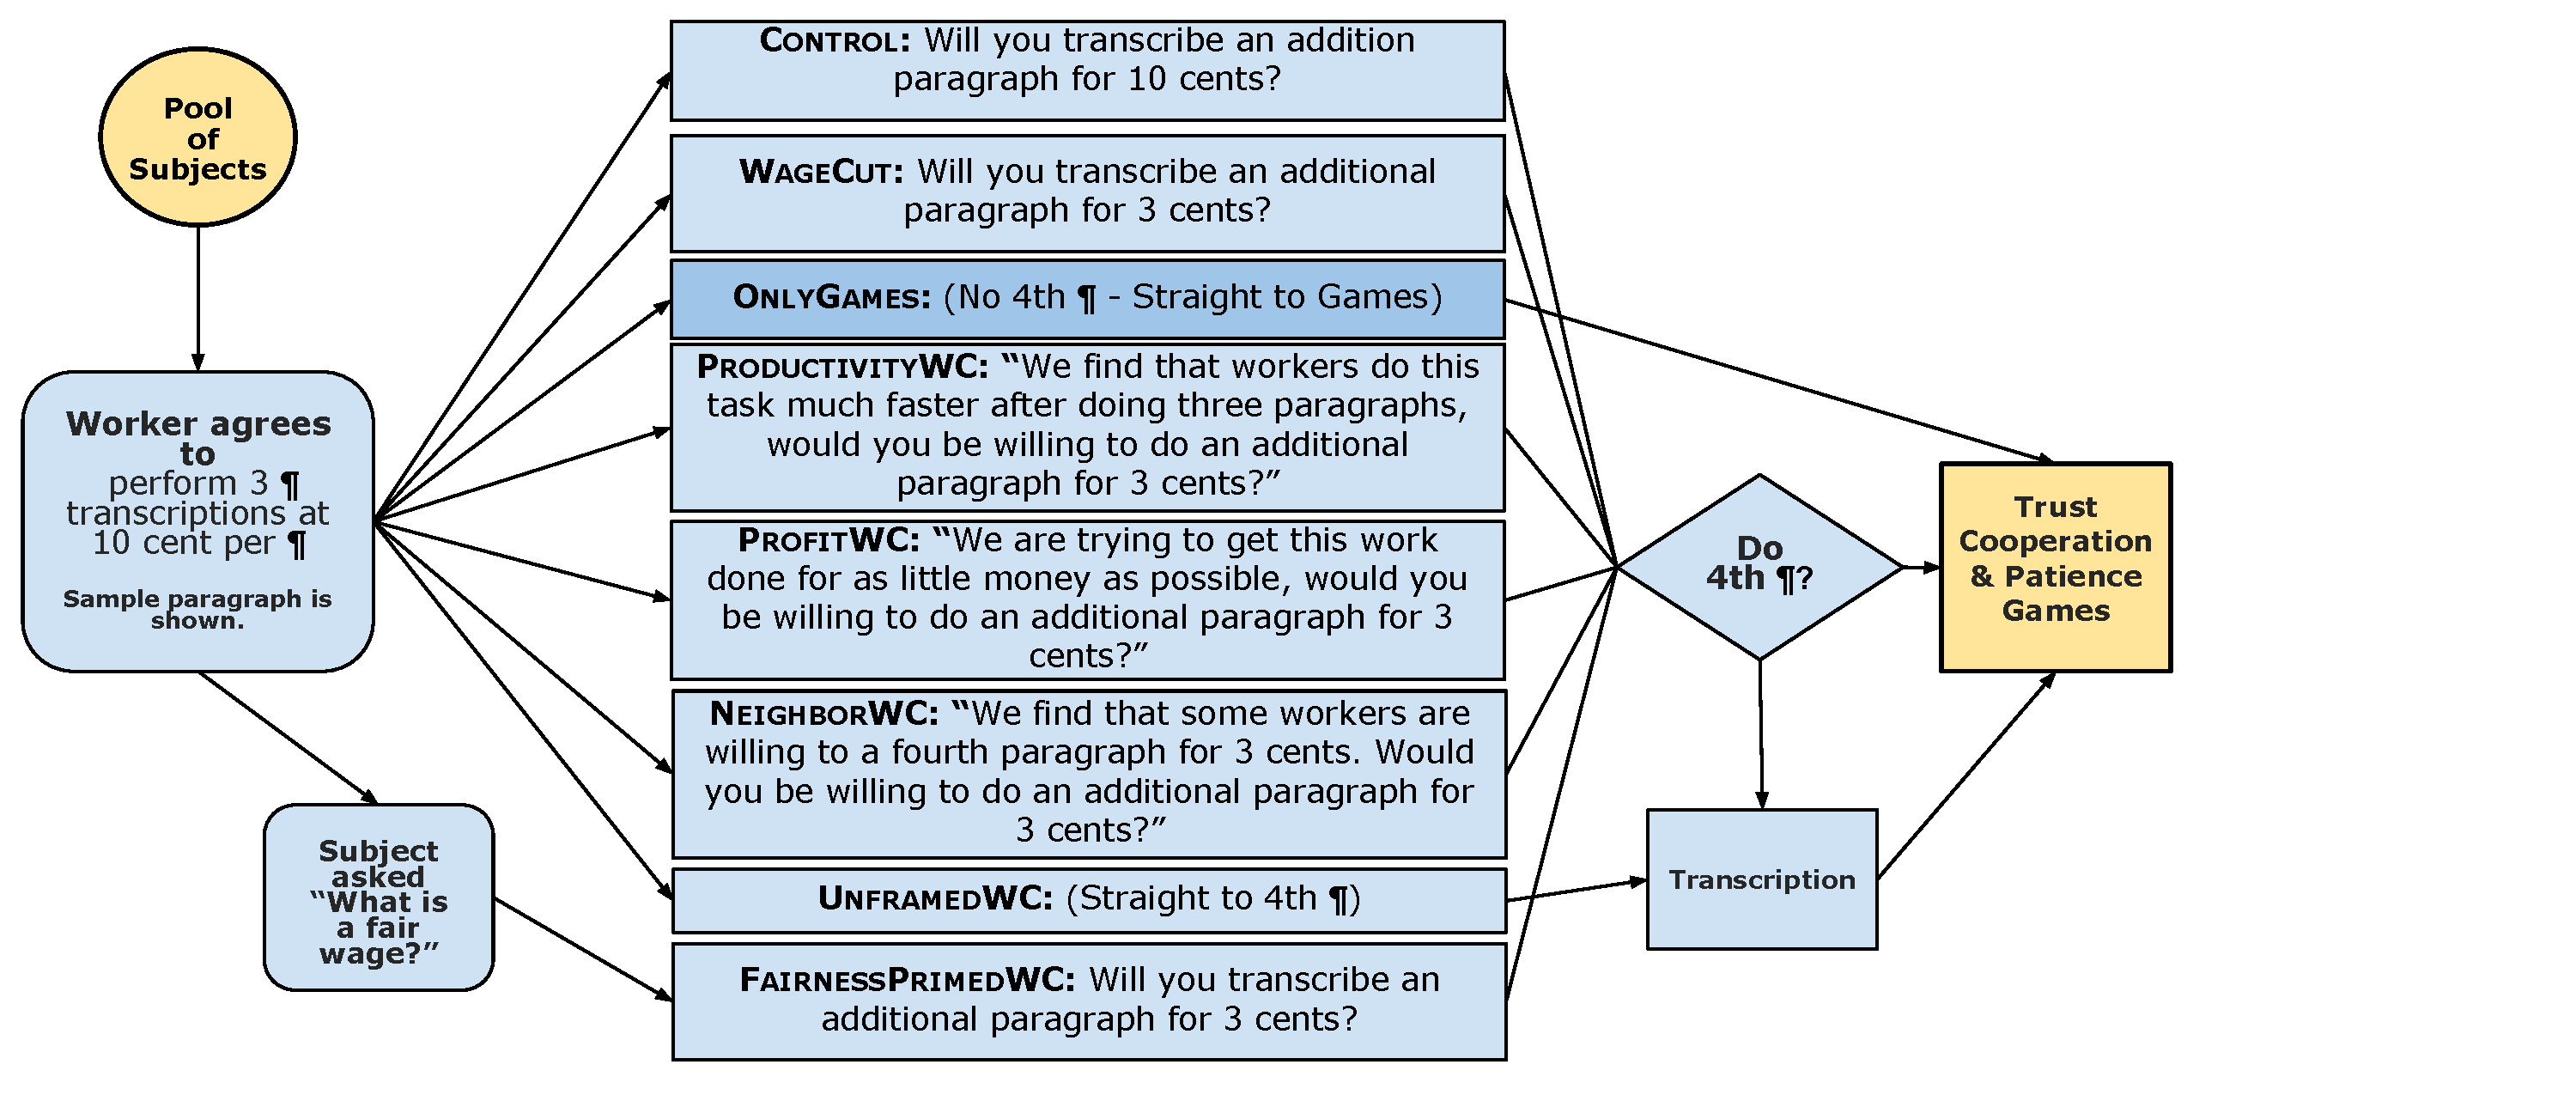
\includegraphics[width = \linewidth]{./media/exp.pdf} 
\\
\footnotesize 
\emph{Notes:} This figure illustrates the flow of subjects through the experiment. 
\end{minipage}
\end{figure}

\begin{figure}[b!]
  \caption{Offer to perform an additional transcription presented to subjects in \textsc{Control} \label{fig:G1}}
\centering
\begin{minipage}{0.85\linewidth}
   \fbox{ 
\includegraphics[width = \linewidth]{../experimental_materials/G1_framing.png} }
\\
\footnotesize \emph{Notes:} After subjects completed the initial three paragraphs, they were, in most cases, presented the offer to do an additional page.
This is a screenshot for offer presented to subjects assigned to \textsc{Control}.
\end{minipage}
\end{figure}
 
\section{Results}

\subsection{Accepting an unexplained wage cut}
We first test whether being offered a lower wage caused fewer workers to accept our offer to transcribe a fourth paragraph.
At a lower offered piece rate, we expected fewer workers to accept the offer, since for some fraction, the marginal cost of doing another transcription outweighs the marginal benefit.
This test cannot distinguish between the sales contract and employment views, but it does let us verify that workers find the task costly and that precise amount offered matters to workers. 
The two relevant experimental cells for this question are \textsc{Control} and \textsc{WageCut}. 
\begin{description}
 \item[\textsc{Control}:] Subjects were offered their previous high wage of 10
  cents to perform an additional transcription.
 \item[\textsc{WageCut}:] Subjects were offered a lower wage of 3 cents to perform an additional transcription.
   No explanation was given for the lower wage offer.
   The precise language of the offer was ``Will you transcribe an additional paragraph for 3 cents?.''
\end{description} 
Table~\ref{tab:uptake_simple} shows that, as expected, substantially fewer workers are willing to transcribe a pararaph when the offered rate is 3 cents instead of 10 cents.

\input{./tables/uptake_simple.tex}

Column~(1) of Table~\ref{tab:uptake_simple} reports an estimate of
\begin{align}
  \textsc{AddPara} = \beta_0 + \beta_{1} \textsc{WageCut} + \epsilon, 
\end{align}
where $\textsc{AddPara}$ is an indicator for whether the worker performed the additional paragraph transcription and \textsc{WageCut} is an indicator that the subject was assigned to that group (we will use this indicator/group name convention throughout the paper). 
The comparison group in the regression is \textsc{Control}. 
In terms of magnitude, we can see that a 70\% reduction in wages (10 cents to 3 cents) led to an approximately 30\% reduction output, implying an elasticity of labor supply of about $0.42$.

In Column~(2), several pre-treatment subject characteristics are added to the regression model.
With these added covariates, the treatment effect increases slightly relative to Column~(1), but this estimate is well within the 95\% confidence interval for the Column~(1) treatment effect, as we would expect for a true experiment. 
There is some evidence that self-reported males were less likely to do the follow-on task, as were those that made a large number of prior errors during the expectation building phase.
However, none of the coefficients are conventionally significant.
We can test for whether there are heterogeneous treatment effects by comparing the Column~(2) regression model with one in which the treatment indicator is interacted with all of the pre-treatment covariates.
When we perform this test, we fail to reject the null hypothesis that the coefficients on the interaction terms are all zero, $(p = 0.414)$, making substantial treatment effect heterogeneity unlikely, at least within the limits of the statistical power available.  

\subsection{Is offer rejection about fairness?}
That fewer workers accept the offer to do an additional task is unsurprising---it is in a sense, over-determined, as it is predicted by both the employment and sales contract views. 
However, we can partially test whether workers have an ``employment-like'' view that a lower wage offer is a contract breach by (1) getting subjects to think about fairness with respect to the task and then (b) presenting them the low wage offer. 
Some subjects were assigned to a cell \textsc{FairnessPrimedWC}, in which they were first asked what would be a fair rate for the task before receiving the 3 cent offer.
Appendix~\ref{experimentalMaterials}, Figure~\ref{fig:priming} shows the interface used to present the ``fairness'' question to users. 
\begin{description}   
\item[\textsc{FairnessPrimedWC:}] Subjects were offered a lower wage of 3 cents to perform an additional task.
No explanation was provided, but we first asked subjects what they thought would be a fair wage for doing an additional task.
\end{description}
For the sake of brevity, we simply describe the results rather than present them in regression tables. 
Comparing acceptances in \textsc{FairnessPrimedWC} to our \textsc{WageCut} cells, acceptance of the offer was 41\% in \textsc{WageCut} and 33\% in \textsc{FairnessPrimedWC}, or an 8 percentage point difference.
Despite this lower uptake when fairness was primed, the standard error for the differences in means is slightly more than 15 percentage points and the p-value of a t-test for a two-sided means comparison is $p=0.63$.
Clearly we cannot reject a null hypothesis of no effect from priming, but the direction of the effect is what we would expect if worker decision making was mediated by fairness concerns (assuming a 3 cent offer after a 10 cent offer would be viewed by most as unfair). 

\subsection{The effects of justifying the wage cut}
Providing some justification for a wage cut might change a worker's probability of accepting that wage cut. 
For example, a ``reasonable'' justification might induce the worker simply to consider the offer relative to their reservation wage for the task. 
In contrast, ``unreasonable'' justifications might even increase the cost of accepting the lower offer.
To return to the question of how we should characterize relationships in this market, in the sales contract view, justifications should be immaterial, because they do not change payoffs, but they would matter in the employment view. 
To test this notion that justifications can alter wage cut acceptance, we randomized subjects to cells with varying justifications. 
\begin{description} 
\item[\textsc{ProductivityWC}:] Subjects were offered a lower wage of 3 cents
  to perform an additional task, but we first informed them that most
  workers can complete tasks more quickly after they gain some experience.
  The precise language was ``We find that workers do this task much faster after doing three
paragraphs, would you be willing to do an additional paragraph for 3
cents?''
\item[\textsc{ProfitWC}:] Subjects were offered a lower wage of 3 cents to
  perform an additional task, but we first informed them that we are trying to
  get as much work done for as little money as possible. The precise language was ``We are trying to get this work done for as little money as
possible, would you be willing to do an additional paragraph for 3
cents?''
\item[\textsc{NeighborWC}:] Subjects were offered a lower wage of 3 cents to
  perform an additional task, but we informed them that in our
  experience, other workers are willing to accept the lower
  offer.\footnote{This was a true statement. From earlier pilot experiments,
    we knew that some subjects were willing to work at this lower wage.} The precise language was ``We find that some workers are willing to do a fourth paragraph
for 3 cents. Would you be willing to do an additional paragraph for 3
cents?'' 
\end{description}

The motivations for \textsc{ProductivityWC} and \textsc{ProfitWC} were to contrast ``reasonable'' and ``unreasonable'' justifications for the wage cut.
Although \textsc{ProfitWC} is unrealistic in the sense that no real firm would propose a wage cut in that manner, it is still a useful treatment in that it lets us test how workers react to an extreme, insulting justification:
\textsc{ProfitWC} tests whether any justification---no matter how insulting---``works.''
Perhaps any justification would be effective---\cite{langer1978mot} showed that asking someone to let you cut in line to make copies ``because you need to make copies'' dramatically increases compliance compared to just asking without the justification.

\textsc{NeighborWC} tests the notion that workers ``learn'' how to react from other workers. 
One reason why \textsc{NeighborWC} might mitigate the behavioral response to a wage cut is that perhaps the psychic cost of taking work below one's past wage comes not just from a fear of being exploited, but also from a fear of being singularly exploited. 
The notion that social comparisons could affect the response to wage cuts has some empirical support---\cite{luttmer2005} found that individuals feel worse-off when others around them earn more.

Consistent with the employment view but not the sale contract view, the empirical results in Table~\ref{tab:uptake_framing} show that justifications do matter, with ``reasonable'' justifications substantially increasing the fraction of workers willing to work at the new, lower piece rate.
Compared to the unexplained cut in \textsc{WageCut}, however, the unreasonable explanation, \textsc{ProfitWC}, did not substantially decrease acceptance, at least within the limits of available statistical power.

\input{./tables/uptake_framing.tex}

We first consider how each justification by itself affected a worker's willingness to perform the fourth transcription at the new rate.  
Column~(1) of Table~\ref{tab:uptake_framing} reports an estimate of 
\begin{align}
  \textsc{AddPara} = \beta_0 + \beta_{1} \textsc{ProductivityWC} + \beta_{2} \textsc{ProfitWC} + \beta_{3} \textsc{NeighborWC} + \epsilon 
\end{align}
where the sample consists of all the justification groups and the unexplained group, with $\textsc{WageCut}$ being the comparison group. 
The coefficient on the productivity justification indicator is positive and conventionally significant, with nearly a 30 percentage point increase in the fraction of workers accepting the lower offer.
The coefficient on the neighbor justification is smaller, with the effect being about 23 percentage points.
It is not conventionally significant, though the difference between the neighbor and the productivity coefficients would itself not be significant.
The profit justification is negative and non-trivial in magnitude---the effect is about an 11 percentage point reduction in task acceptance---but it is far from conventionally significant.
In Column~(2), the outcome is the same, but we pooled what we considered ``reasonable'' justifications, \textsc{ProductivityWC} and \textsc{NeighborWC}, and compared them to what we considered unreasonable or missing justifications, \textsc{WageCut} and $\textsc{ProfitWC}$. 
Here the difference is stark, with the reasonable justifications increasing output by nearly 30 percentage points.
This greater effect is attributable to the roughly similar magnitudes for the coefficients on \textsc{NeighborWC} and \textsc{ProductivityWC} and the negative and fairly large coefficient on the profit justification indicator. 

\subsection{The effects of explicitly asking about task continuation}
One of the key differences between the sales and employment contract is that in the employment contract, the expectation is that the project will continue until explicitly dissolved.
In contrast, the sales contract is ended when the specified task is completed.
We wanted to test whether simply presenting workers the additional transcription task, labeled with the new 3-cent wage, would cause a different reaction from workers, relative to flagging the proposed explicitly new wage and requiring workers to give a yes or no answer to whether they wanted to continue.
To test whether this offer framing mattered, we created a cell \textsc{UnframedWC}. 

\begin{description} 
\item[\textsc{UnframedWC}:] Subjects were \emph{not} explicitly offered a lower
  wage to perform an additional task. Rather, they were simply brought
  to the next task, which was clearly labeled with the new, lower wage
  of 3 cents.  There was a button at the bottom of the screen that
  allowed them to quit and continue to the follow-on contextualized
  games.
\end{description} 
Consistent with the employment contract view, Table~\ref{tab:uptake_unframed} shows that this ``unframed'' wage cut was remarkably effective, in that all subjects assigned to \textsc{UnframedWC} transcribed the fourth paragraph.  

\input{./tables/uptake_unframed.tex}

First we consider output in the unframed cell relative to the explicit, unjustified wage cut of \textsc{WageCut}. 
Column~(1) of Table~\ref{tab:uptake_unframed} reports an estimate of 
\begin{align}
  \textsc{AddPara} = \beta_0 + \beta_{1} \textsc{UnframedWC} + \epsilon.
\end{align}
The comparison group is \textsc{WageCut}, the unexplained wage cut. 
The coefficient on the ``unframed'' indicator shows that not explicitly framing work continuation as a choice leads to very high acceptance of the wage cut:
in fact, 100\% of subjects in \textsc{UnframedWC} performed the follow-on paragraph transcription, compared to just a little more than 40\% of subjects in \textsc{WageCut}.  
Column~(2) reports the same regression as Column~(1), but with the comparison group being the \textsc{Control} group instead of \textsc{WageCut}.
When we compare the unframed wage cut group to the subjects that had no wage cut at all, we can see that the unframed group had about a 25 percentage point increase over those not receiving a wage cut at all. 
In other words, not framing a decision to continue working led to far more output than even offering the previous rate.

There are several possible interpretations of these results. 
It is possible that subjects failed to consider their option of refusing to do the task by simply entering a poor transcription (the most extreme form being leaving the text box blank).  
Another possibility is a worker might believe they were in error: if a worker thought she had read the instructions incorrectly, she might worry that a skipped transcription would jeopardize payment for work already completed.
Beyond just payment, workers might worry about their reputation.
MTurk does have a rudimentary reputation system, in that buyers can ``reject'' a worker's submission and future buyers can screen workers ex ante based on their rejection rates, making rejections consequential.
However, there is no rich reputation system with bilateral feedback and non-binary rating options common in other electronic commerce sites \citep{dellarocas2006reputation}, including in other online labor markets \citep{moreno2014}. 

These caveats aside, the evidence does suggest that explicitly flagging a wage change has a different effect than imposing the same change surreptitiously. 
If workers regard their relationships with the buyer as an employment contract, this continuation of work---without any explicit discussion of prices or decisions---is what they would expect to happen normally.
In contrast, a worker with the sales contract view who was told ex ante he would perform three paragraphs would be very surprised by an additional task, as the contract was at that point dissolved. 

\subsection{Comparison of output by offer size, justification and explicitness of follow-on offer}
The pattern of output results can be more clearly seen in Figure~\ref{fig:response}. 
We have divided reasons into ``reasonable'' and ``non-reasonable'' with ``reasonable'' based on our own judgment. 
The plots show that reasonable justifications keep output levels quite close to those in the 10-cent offer \textsc{Control} group.
The remarkable uptake in \textsc{UnframedWC} is also apparent, as well as the much lower output in the cells with no justification or an unreasonable justification. 

\begin{figure}
  \caption{Fraction of subjects accepting the offer to perform an additional transcription task \label{fig:response}} 
\centering
\begin{minipage}{0.85 \linewidth}
    \includegraphics[width = \linewidth]{./plots/uptake.pdf}
\\
\footnotesize
\emph{Notes:} For each point estimate, we include the 95\% CI, calculated using the Wilson method for a binary proportion.  
\end{minipage}
\end{figure}   

\subsection{Follow-on task performance}
Workers might be willing to ``accept'' a wage cut and then retaliate by offering poor performance on the task, such as by introducing many errors in the transcription.
This is the consensus view for why firms are so averse to cutting wages. 
In our experimental setting, detecting retaliation is challenging because of selection.
We know that the different cells have different task acceptance rates. 
As such, any differences in follow-on error rate could reflect some combination of selection and treatment.
We can potentially deal with this selection problem by controlling for transcription quality from the first phase of the experiment. 
It is the case that error rates in the fourth paragraph are highly correlated with the error rate in the initial three paragraphs: 
when pooled, the point estimate of the correlation coefficient is $\rho = 0.33$ and a 95\% confidence interval of $[0.14, 0.56]$.\footnote{
  Standard errors for the correlation coefficient were calculated with one million bootstrap replications.
}

Table~\ref{tab:errors} shows that there is no evidence that workers willing to accept the wage cut were any worse overall, relative to \textsc{Control}.
However, there is some evidence that workers assigned to the unreasonable \textsc{ProfitWC} produced worse transcriptions, even when controlling for output quality during the first phase of the experiment. 
However, it is important to remember that even with our prior error controls, we cannot credibly estimate causal effects.

\input{./tables/error.tex}

First, we test whether workers assigned any of the wage cut cells had worse performance compared to those who were offered their previous rate.
Column~(1) of Table~\ref{tab:errors} reports an estimate of 
\begin{align}
  \log \textsc{EditDist}^4 = \beta_0 + \beta_1 \textsc{AnyWageCut} + \log \sum_{k \in \{1,2,3\}} \textsc{EditDist}^k + \epsilon,
\end{align}
where $\textsc{EditDist}^4$ is the edit distance for the fourth paragraph and \textsc{AnyWageCut} is an indicator that the subject was assigned to any of the wage cuts groups.
Note that we control for the log cumulative error in the first three paragraphs, which should at least partially address the possibility that selection effects drive differences in error rates.  
The coefficient on \textsc{AnyWageCut} is negative---implying fewer errors---but is also imprecisely estimated and far from conventionally significant.

In Column~(2), we decompose \textsc{AnyWageCut} into the indicators for the different cells and use \textsc{WageCut} as the comparison group.
This lets us test whether any of the framings or justifications among workers accepting the wage cut affected output.
Here we see that the coefficient on \textsc{ProfitWC} is large and positively significant, with nearly a 50\% higher error rate.
This is suggestive evidence that workers in the profits justification retaliated, but there are two important caveats.
First, this group  had the lowest acceptance rate and so any selection effects would be particularly strong for this group.
Second, we are looking at five different treatment cells and only one is conventionally significant.
On the other hand, for theory reasons, we also have reason to believe that if there was retaliation, it would be more likely in \textsc{ProfitWC}. 

\section{Conclusion} 
Our main positive finding is that framing can strongly affect the behavioral response to a wage change.  
Workers reduce output---and possibly work quality---when wages are cut for capricious or selfish-seeming reasons, but workers do not reduce output as much and apparently are still willing to cooperate if the employer has seemingly valid reasons for his or her actions.
Workers on MTurk exhibit the same fairness-mediated reactions to wage cuts thought to characterize worker reactions to wage cuts in conventional employment relationships.
Further, the results from the ``unframed'' wage cut experiment suggest that workers have a bias towards simply continuing to work rather than viewing the completion of the last agreed-upon task as the end of the contract.
While this is not the only interpretation, it is some evidence towards the employment characterization of the relationships that are created (at least from the worker's perspective). 
As such, it seems unlikely that firms hiring in online labor markets can treat their interactions as spot-market transactions, but must instead consider the quasi-employment nature of the relationships they seem to create.

An interesting question for future research is to what extent this employment-like characterization makes an economic difference in what can and cannot be done in which kinds of markets.
The existence---and to date, persistence---of very different kinds of platforms for online work seems to indicate that having a variety of platforms is useful for different purposes, but each raises its own challenges.  
For example, \cite{boudreau2011incentives}, looking at paid programming contests, illustrates the power of the ``open call'' format for certain kinds of problems, in that the probability of solution rises with more entrants, and yet the contest version of a wage cut---adding more competitors---can reduce incentives.
They show that for highly uncertain problems, the payoff to adding more competitors dominates, but not for more well-specified projects.
If sufficiently well specified and certain, the innovation ``contest'' of one---a single hired worker might dominate.  
Going back to our MTurk domain, for certain kinds of problems, an employee-like mindset is desirable, as the high-powered incentives in a sales contract can motivate workers towards both cost savings (good) but also corner-cutting and opportunism (bad).

Our results come from MTurk, which is just one of several online labor markets.\footnote{
  Other markets include Upwork (the combined marketplace of the merged oDesk and Elance marketplaces), Freelancer.com, Fiver, 99Designs and several others.
}
However, some of the characteristics that MTurk exhibits in the extreme---very short-lasting relationships, relatively small stakes, computer-mediated work relationships---are appearing in a variety of labor markets.
In recent years, we have seen the rise of new forms of computer-mediated marketplaces, including Uber, Lyft, TaskRabbit, Handy, Instacart, and so on, that share some similarities. 

These markets are are capturing so much attention because they raise so many questions.
On the positive side, the greater flexibility they offer workers seems valuable, expanding the set of options available to workers.
It is an open research question as to how much value workers place on the flexibility these kinds of markets afford them---the ability to work when they want, at terms that they set.
On the negative side, these markets have received criticism for potentially transferring power away from individual workers and putting them more at the whim of the platform of would-be buyers.  
More research on the nature of the relationships created in these platforms and the larger implications of online work is needed. 


\bibliographystyle{aer}
\bibliography{wages_of_paycuts.bib}

\appendix 

\newpage

\section{Consummate performance measures} \label{sec:games}
When we designed the experiment, we also wanted to look for other indications of work effort and cooperation beyond just acceptance of the wage cut.
To that end, we had subjects play a number of contextualized games to measure ``consummate performance.''
This part of the experiment had generally uninteresting results---in part because of the relatively low power of the design to detect anything but very large effects.
We do present the results here in an appendix for the benefit of interested parties and for completeness. 

\subsection{Consummate performane measures}
To measure consummate performance, subjects played a collection of contextualized games that we hoped would not seem unusual to the subjects.
These games tried to measure worker patience, trust in us, and cooperation with us. 
To measure patience, we simply asked subjects whether they would be willing to forgo nearly immediate payment in exchange for a 30-cent bonus to be paid out in two weeks. 

We measured trust with a modified version of the trust game \citep{glaeser2000}.
Subjects were told to imagine they had \$15 and that they could choose any fraction of that money to ``send'' to us. 
If we judged their work favorably, we would double what they sent and ``send it back''; in the event of an unfavorable judgment, we would keep whatever they sent.\footnote{
  The subject we randomly selected had chosen to send the full \$15; we gave him or her \$30.
} 
The instructions and interface are shown in Appendix~\ref{experimentalMaterials}, Figure~\ref{fig:trust}. 
To save money, we told subjects that we would select one player at random and implement his or her choices. 
Although this game measures the worker's trust in us (e.g., trust that we will follow our own protocol and judge their work fairly), it is confounded with the worker's confidence, risk aversion and beliefs about our standards for the
work. 
If these non-trust factors held constant across experimental groups, we could in principle detect changes in trust, though this assumption of constant effects is questionable.
In any event, these factors should be unaffected by the treatment for the subjects in a cell we created in which subjects proceeded immediately to the games. 

We measured cooperation in two ways: (a) willingness to give free advice and (b) willingness to take a short survey at a later date.
For the first cooperation measure, subjects were asked to suggest ways to make the transcription task easier.
The wording of the request made it clear that offering advice was voluntary and that no payment would be made for the offered advice.\footnote{
  The text of the actual question was, ``Please help us make these tasks easier for other workers. Describe what steps workers can take to make doing these transcriptions easier.''} 
The instructions and interface are shown in Appendix~\ref{experimentalMaterials}, Figure~\ref{fig:advice}. 
For a second cooperation measure, we offered subjects the opportunity to take a follow-on survey for an additional 15 cents.\footnote{
  When you pay workers on MTurk, you can embed a short message about why you are paying them---we embedded the link to our survey in this message.
  Remarkably, not one person who agreed to do the survey actually did it after we sent them the link.
  We had intended to use completing the survey as another measure of cooperation and trustworthiness, but there was no variation in survey response.
  Given the universal rejection, we fear that some technical problem may have prevented completion.
} 

The instructions and interface for the survey request are shown in Appendix~\ref{experimentalMaterials}, Figure~\ref{fig:follow_on_survey}. 

\subsection{Consummate performance results} 
In addition to simply not accepting a wage cut or doing a poor job, workers who face wage cuts could withhold ``consummate'' performance. 
Consummate performance is difficult to measure---at least in some models, the difficulty of measuring (or at least contracting upon it) is definitional.
These challenges aside, we attempted to measure consummate performance with the ``games'' phase of the experiment, which followed treatment.
Each game was designed to give workers the chance to evince some changed attitude towards us that a real employer might find consequential. 
The games are all described in Section~\ref{sec:games}. 
To aid in the comparison across groups, we created a cell in which subjects were not exposed to an offer to perform an additional paragraph transcription. 
\begin{description}   
\item[\textsc{OnlyGames}:] Subjects were not offered an additional task.
  After the initial transcriptions, they went straight to the follow-on games.
\end{description}
We had hoped that our consummate measures would all be highly correlated with each other, suggesting that the different measures were all manifestations of the same positive or negative change towards us as an employer/trading partner. 
However, there is only weak evidence that this hope was borne out: 
Table~\ref{tab:cor} shows the correlation matrix for the four consummate performance measures, pooled across all experimental groups.
We see that the patience measure had no strong relationship to any of the other measures and is even slightly negatively correlated with the advice measure.
The advice and trust measures are positive related, as are survey and advice measures---but survey and trust are not related to each other. 

\input{./tables/cor.tex}

The first question about the any of the games is whether simply being asked to perform an additional paragraph transcription had any effect.
For this, we can compare \textsc{Control}, which received a 10-cent offer, to the \textsc{OnlyGames} group.
Column~(1), Table~\ref{tab:games} reports an estimate of 
\begin{align}
  \textsc{Survey} = \beta_0 + \beta_{1} \textsc{Control} + \epsilon 
\end{align} 
where the sample consists of subjects in \textsc{Control} and the excluded group is \textsc{OnlyGames}.
We can see that subjects that were presented an additional fourth paragraph were about 9 percentage points less likely to agree to a survey compared to those simply brought directly to the games.
However, this estimate is not conventionally significant. 
Note that among \textsc{OnlyGames}, agreement to do the survey was 100\%. 
For the other games, we also find no evidence of a differential performance:
in two-sided t-tests for both the advice z-score and the trust z-score, we fail to reject the null hypothesis of no difference in group means, with $p = 0.29$ and $p = 0.174$, respectively.
Furthermore, the \textsc{Control} coefficient is positive for the trust and advice measures. 

Next we test whether any wage cut---regardless of how framed or justified---affected willingness to take the survey. 
Column~(2) reports an estimate of 
\begin{align}
  \textsc{Survey} = \beta_0 + \beta_1 \textsc{AnyWageCut} + \epsilon,  
\end{align} 
where \textsc{AnyWageCut} is an indicator that the subject was assigned to \textsc{WageCut} of any of the four wage cut groups. 
The comparison group is the \textsc{Control} group, to which the 10 cent offer was made. 
The coefficient on \textsc{AnyCut} is very close to zero, implying no detectable effect on willingness to take the survey.
As before, for the other games, we also find no evidence of a differential performance:
in two-sided t-tests for both the advice z-score and the trust z-score, we fail to reject the null hypothesis of no difference in group means, with $p = 0.26$ and $p = 0.67$, respectively.

\input{./tables/games.tex}

Despite no overall effect of a wage cut, we know that the different justifications strongly affected willingness to accept the wage cut. 
To test whether these justifications affected consummate performance, Column~(3) reports a regression where \textsc{AnyWageCut} is decomposed into each of the distinct justifications, with \textsc{WageCut} as the comparison group.  
In this regression, we see that the coefficient on \textsc{ProfitWC} is negative and large, with a nearly 20 percentage point reduction in agreement to complete the survey.
The effect is conventionally significant.
However, given the multitude of treatment cells, the finding of one significant effect out of five could very likely be due to chance.
On the other hand, finding the strongest negative effects in the cell with the most unreasonable justification could indicate an actual behavioral response.
And yet there is additional evidence for the argument that the seeming effect of the profits treatment is spurious:
in Columns~(4) and (5), we change the outcomes to the advice and trust z-scores and find no substantial differences across cells.
For both outcomes, we would fail to reject the null hypothesis of zero coefficients on all group indicators ($p = 0.16$ for the advice measure and $p=0.74$ for the trust measure).
However, for both the trust and advice measures, we are under-powered to detect anything but very large effects, with the standard errors being more than 3/10ths of a standard deviation in the outcome variable.

\section{Experimental materials} \label{experimentalMaterials}

The actual surveys used for each of the experimental groups are hosted at the following URLs: 
\begin{itemize}
\item \textsc{Control}: \href{http://www.surveymonkey.com/s/R23DT7Y}{http://www.surveymonkey.com/s/R23DT7Y}
\item \textsc{WageCut}: \href{http://www.surveymonkey.com/s/R23FZHW}{http://www.surveymonkey.com/s/R23FZHW} 
\item \textsc{OnlyGames}: \href{http://www.surveymonkey.com/s/R2G53NM}{http://www.surveymonkey.com/s/R2G53NM} 
\item \textsc{ProductivityWC}: \href{http://www.surveymonkey.com/s/R2BXXM7}{http://www.surveymonkey.com/s/R2BXXM7} 
\item \textsc{ProfitWC}: \href{http://www.surveymonkey.com/s/R2H6QQ2}{http://www.surveymonkey.com/s/R2H6QQ2} 
\item \textsc{NeighborWC}: \href{http://www.surveymonkey.com/s/R2HMWZR}{http://www.surveymonkey.com/s/R2HMWZR} 
\item \textsc{UnframedWC}: \href{http://www.surveymonkey.com/s/R2699DW}{http://www.surveymonkey.com/s/R2699DW} 
\item \textsc{FairnessPrimedWC}: \href{http://www.surveymonkey.com/s/R2Z2SH9}{http://www.surveymonkey.com/s/R2Z2SH9} 
\end{itemize} 

\begin{figure}[!h] 
  \caption{Initial instructions page\label{fig:instructions}}
\centering
\begin{minipage}{0.85\linewidth}
   \fbox{
\includegraphics[width = \linewidth]{../experimental_materials/landing_page.png} }
\\
\footnotesize 
\emph{Notes:} This was the first page that all participants---regardless of experimental group---first landed on. 
\end{minipage}
\end{figure}

\begin{figure}
  \caption{Transcription environment for all paragraphs \label{fig:environment}}
\centering
\begin{minipage}{0.85\linewidth}
   \fbox{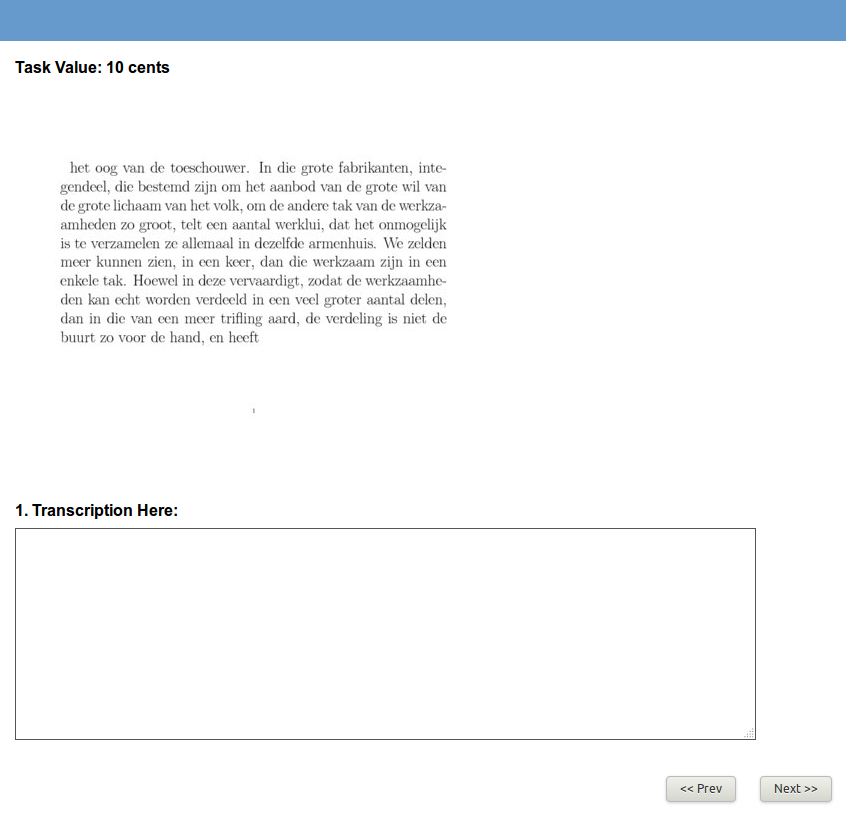
\includegraphics[width = \linewidth]{../experimental_materials/paragraph.png} }
\\
\footnotesize 
\emph{Notes:} All subjects transcribing paragraphs used this
interface for both the initial three paragraphs and the additional
paragraph. Note that the task value differed depending upon the
treatment assignment.
\end{minipage}
\end{figure}

\begin{figure}
  \caption{Fairness priming question in \textsc{FairnessPrimedWC} \label{fig:priming}}
\centering
\begin{minipage}{0.85\linewidth}
   \fbox{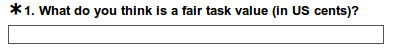
\includegraphics[width = \linewidth]{../experimental_materials/prime.png} }
\\
\footnotesize 
\emph{Notes:} Subjects in \textsc{FairnessPrimedWC} were asked what was a fair wage for a
paragraph, using this dialog.  
\end{minipage}
\end{figure}

\begin{figure}
  \caption{``Trust game'' dialog \label{fig:trust}}
\centering
\begin{minipage}{0.85\linewidth}
   \fbox{ 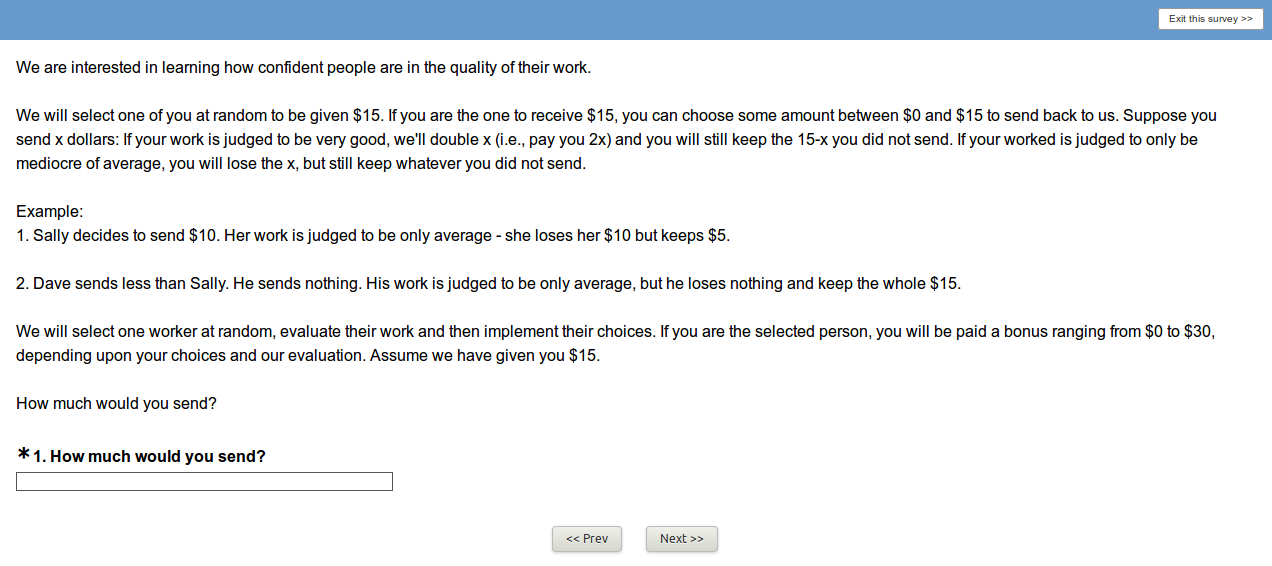
\includegraphics[width = \linewidth]{../experimental_materials/trust_game.png} }
\\
\footnotesize \emph{Notes:} This screenshot shows the instructions and
choices for subjects playing the contextualized ``trust game.''  
\end{minipage}
\end{figure}


\begin{figure}
  \caption{Follow-on survey dialog \label{fig:follow_on_survey}}
\centering
\begin{minipage}{0.85\linewidth}
   \fbox{ 
\includegraphics[width = \linewidth]{../experimental_materials/follow_on_survey.png} }
\\
\footnotesize \emph{Notes:} This screenshot shows the interface in
which we presented subjects with the opportunity to take a follow-on
survey at a later date.   
\end{minipage}
\end{figure}

\begin{figure}
  \caption{``Patience'' dialog \label{fig:patience}}
\centering
\begin{minipage}{0.85\linewidth}
   \fbox{ 
\includegraphics[width = \linewidth]{../experimental_materials/patience.png} }
\\
\footnotesize \emph{Notes:} This screenshot shows the interface in
which we presented subjects with the opportunity to delay getting paid
in exchange for a larger payment at a later date. 
\end{minipage}
\end{figure}

\begin{figure}
  \caption{``Advice'' dialog \label{fig:advice}}
\centering
\begin{minipage}{0.85\linewidth}
   \fbox{ 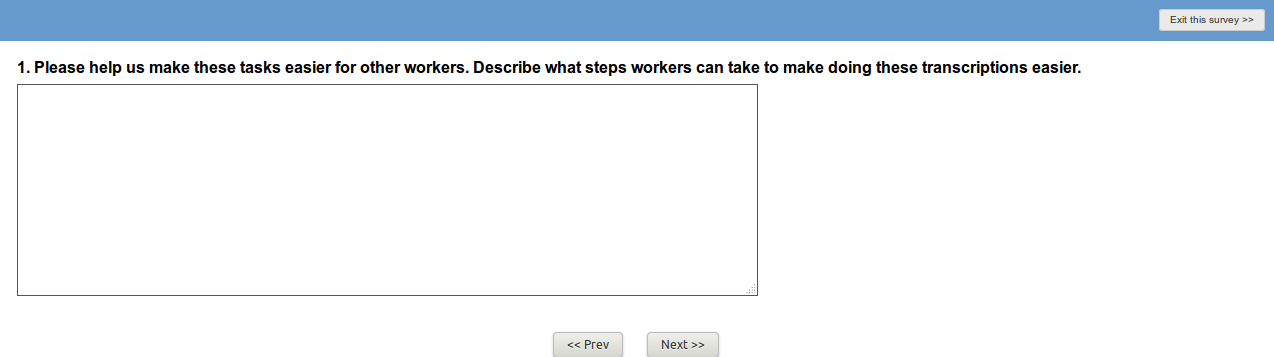
\includegraphics[width = \linewidth]{../experimental_materials/advice.png} }
\\
\footnotesize \emph{Notes:} This screenshot shows the interface in
which we asked subjects to provide advice to other workers. 
\end{minipage}
\end{figure}

\begin{figure}
  \caption{Demographics dialog \label{fig:demographics}}
\centering
\begin{minipage}{0.85\linewidth}
   \fbox{ 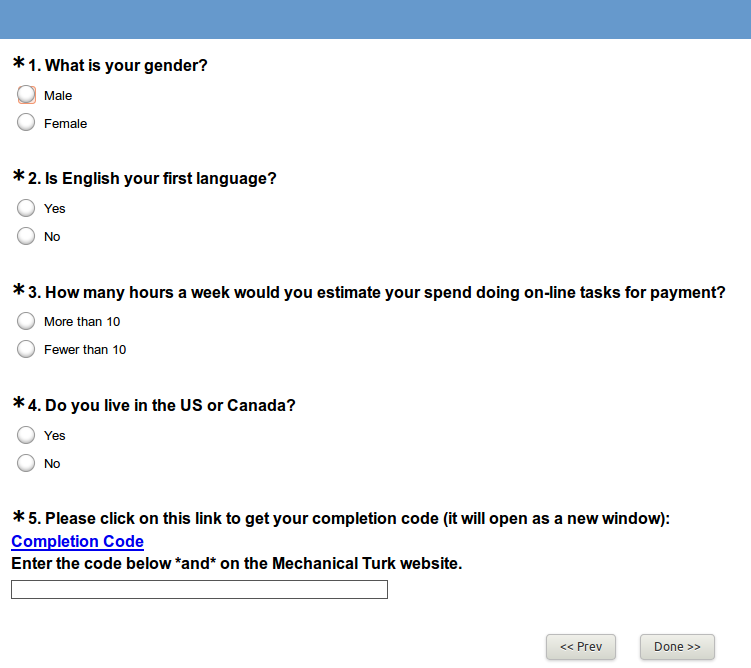
\includegraphics[width = \linewidth]{../experimental_materials/demographics.png} }
\\
\footnotesize \emph{Notes:} This screenshot shows the interface in
which we asked subjects to provide some demographic information. It
also shows the completion code link that subjects used to generate
a code which could link their responses to their MTurk identities. 
\end{minipage}
\end{figure}

\begin{figure}
\centering 
\caption{MTurk tasks that Amazon supports via pre-made templates and vetted workers \label{mturk_proof}}
\begin{minipage}{.85\linewidth}
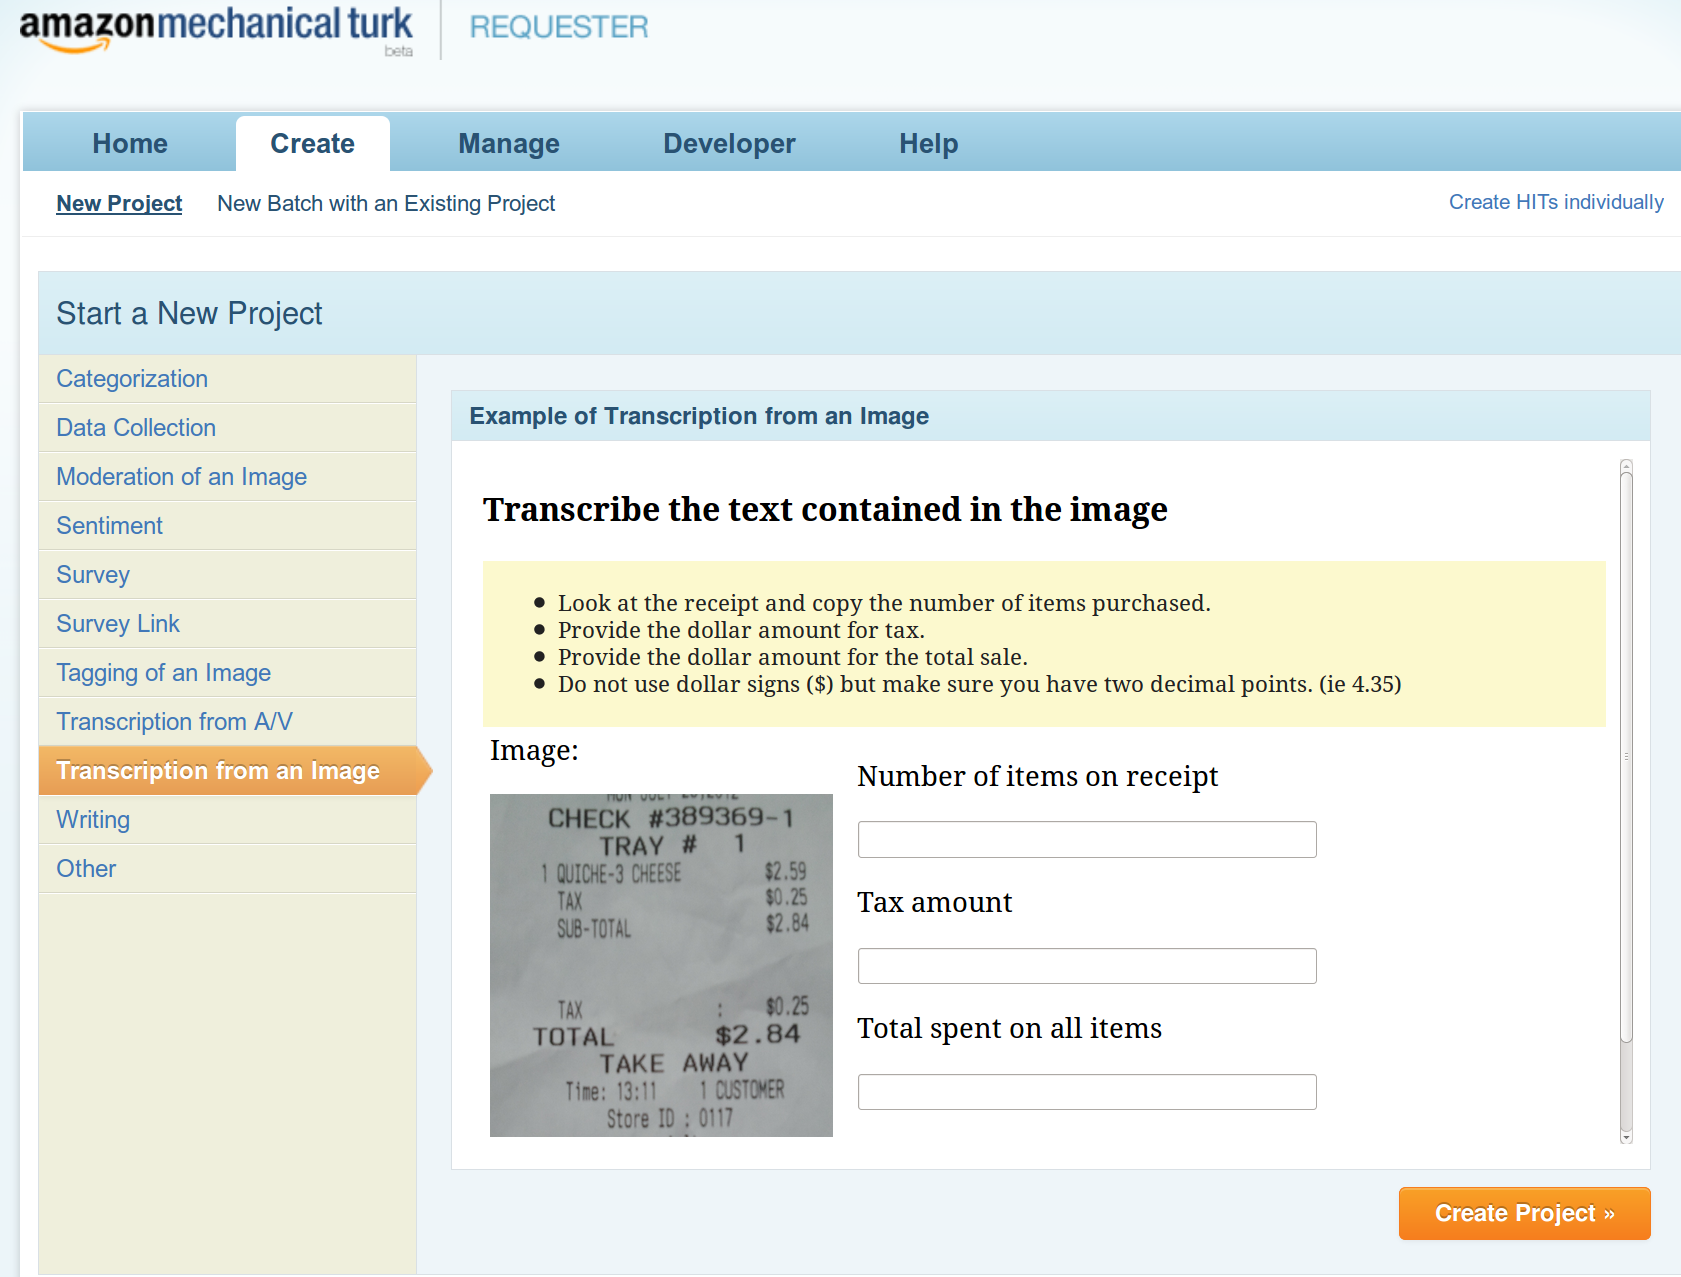
\includegraphics[width = \linewidth]{./images/canonical_mturk_projects.png} 
\\
\footnotesize 
\emph{Notes:} This is a screenshot of the Amazon Mechanical Turk interface for starting a new project from a template. 
The column of text on the left side of the image shows the common use cases for MTurk. 
The ``Transcription from an Image'' task is selected and shown, which is the kind of task we used for our experiment.  
\end{minipage} 
\end{figure} 

\end{document}
